\documentclass[aspectratio=169]{beamer}

\usepackage[utf8]{inputenc}
\usepackage{array}
\usepackage{booktabs}
\usepackage{bold-extra}
\usepackage{graphics}
\usepackage{hyperref}
\hypersetup{%
  colorlinks=true,
  linkcolor=blue,
  filecolor=blue,
  urlcolor=cyan,
}
\usepackage{listings}
\usepackage{multicol}
\usepackage{multirow}
\usepackage[absolute,overlay]{textpos}
\usepackage{setspace}
\usepackage{verbatim}
\usepackage{fancyvrb} % for verbatim centering
\usepackage{tikz}

\usetheme{Warsaw}
\usecolortheme{beaver}
\definecolor{clOrange}{HTML}{E76600}
\definecolor{clAlmostWhite}{HTML}{FEFFD9}
\definecolor{clGreen}{HTML}{007F00}
\definecolor{clFlag}{HTML}{D33682}
\definecolor{clFlagOpt}{HTML}{CB4B16}
\definecolor{clRedFlag}{HTML}{DC322F}
\definecolor{clViolet}{HTML}{4c0070}

\definecolor{clCodeBlue}{rgb}{0.0, 0.18, 0.38}
\definecolor{clCodeGreen}{rgb}{0.0, 0.27, 0.15}
\definecolor{clCodeRed}{rgb}{0.63, 0.0, 0.0}


\setbeamertemplate{navigation symbols}{}
\setbeamercolor{title}{fg=black}
\setbeamercolor{author}{fg=clAlmostWhite}
\setbeamercolor{date}{fg=clAlmostWhite}
\setbeamerfont{author}{size=\huge}
\setbeamerfont{date}{size=\Large}

\newcommand{\greenemph}[1]{\textit{\textcolor{clGreen}{#1}}}
\newcommand{\cpp}[1]{\texttt{\textbf{\textcolor{clCodeBlue}{#1}}}}

\newcommand\fontV{\fontsize{5}{5}\selectfont}

\lstset{
  language=C++,
  basicstyle=\ttfamily,
  keywordstyle=\color{clCodeBlue}\ttfamily,
  stringstyle=\color{clCodeGreen}\ttfamily,
  commentstyle=\color{clCodeRed}\ttfamily,
  morecomment=[l][\color{magenta}]{\#}
}

\title[Friends\#21 :: \cpp{ValueAndReferenceSemantics}]{Value semantics and reference semantics\\
in \cpp{C++} and other languages
}
\author{Adam Graliński}
\date[July'22]{\textbf{\texttt{\color[HTML]{d33682}C++} {\color[HTML]{268bd2}F}{\color[HTML]{2aa198}r}{\color[HTML]{859900}i}%
{\color[HTML]{cb4b16}e}{\color[HTML]{dc322f}n}{\color[HTML]{6c71c4}d}{\color[HTML]{b58900}s}, July 2022}}

\begin{document}

{\usebackgroundtemplate{%
 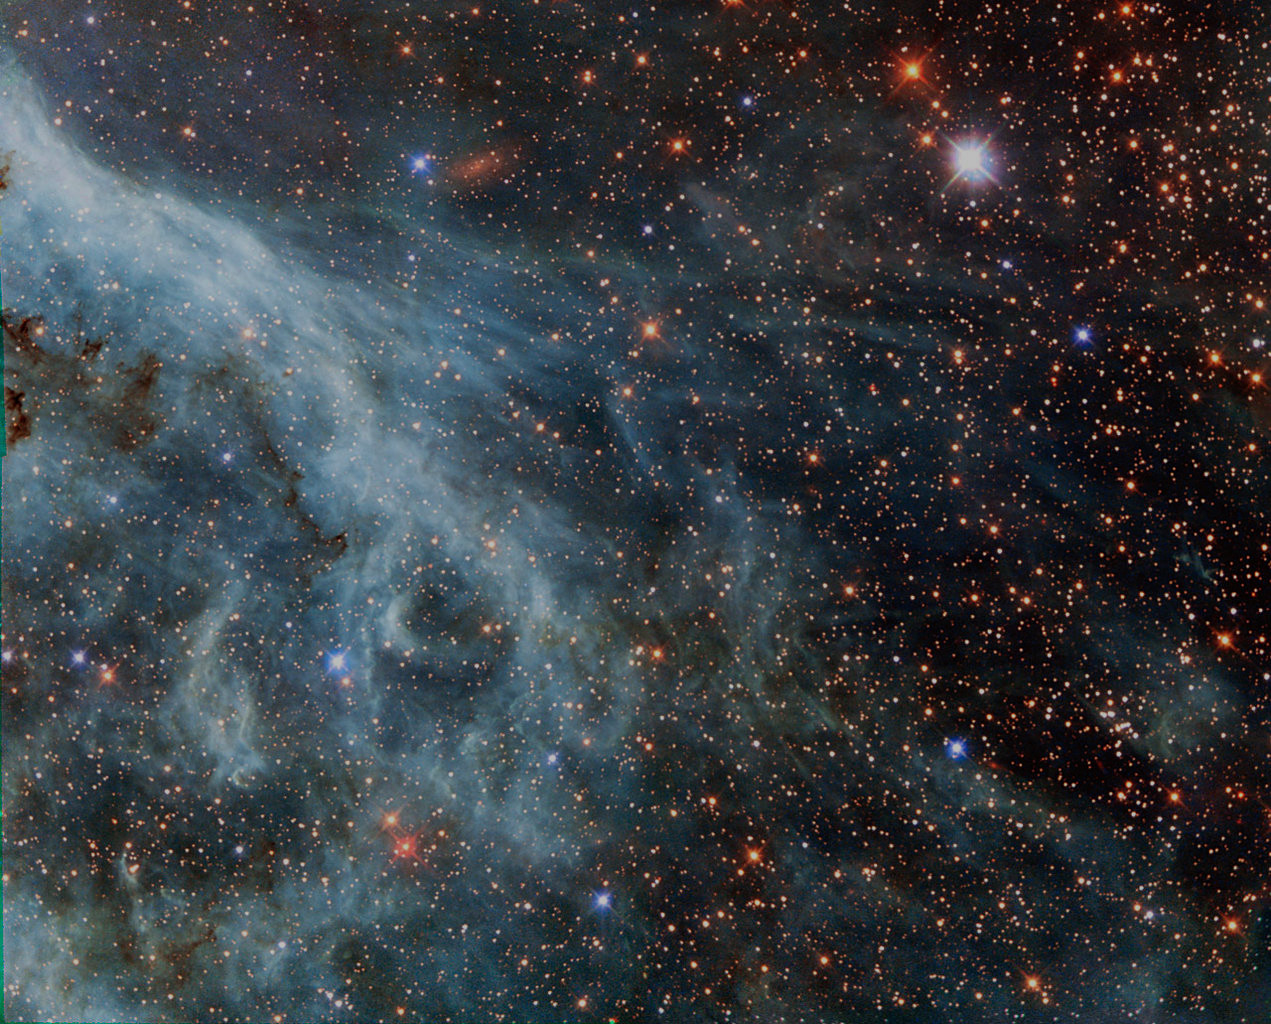
\includegraphics[width=\paperwidth,height=\paperheight]{../common/bg_galaxy.jpg}}
\begin{frame}
\titlepage{}
\end{frame}
}

\begin{frame}
\frametitle{Value semantics and reference semantics}
\begin{center}
  \begin{tabular}{m{6cm} | m{7cm}}
    \textbf{Value semantics} & \textbf{Reference semantics}\\
    \hline{}
    Refers to concrete objects          & Refers to any type-like object\\
    (one specific location in memory)   & held anywhere in memory\\
    \hline{}
    Comparison based on values          & Comparison based on memory addresses\\
    \hline{}
    Deep copying, deep assignment       & Shallow copying, shallow assignment\\
  \end{tabular}
\end{center}
\cpp{C++} uses \greenemph{value semantics} for most things* by default.
\end{frame}

\begin{frame}[fragile]
\frametitle{Semantics for primitive types: \cpp{C++}}
\begin{columns}[T]
  \begin{column}{0.6\textwidth}<1->
    {\color[HTML]{cb4b16}
    \texttt{\textbf{01\_primitives.cpp}}\vspace{-9pt}
    \rule{\linewidth}{2pt}}%
    {\fontsize{8}{6} \lstinputlisting[showstringspaces=false]{code/01_primitives.cpp}}%
    \vspace{-12pt}{\color[HTML]{cb4b16}\rule{\linewidth}{2pt}}%
  \end{column}
  \begin{column}{0.3\textwidth}<2->
    {\color[HTML]{002b36}
    \texttt{\textbf{output}}\vspace{-9pt}
    \rule{\linewidth}{2pt}}%
    {\fontsize{8}{6} \begin{lstlisting}[showstringspaces=false]
b == 10
value semantics
for primitives
    \end{lstlisting}
    }
    \vspace{-12pt}{\color[HTML]{002b36}\rule{\linewidth}{2pt}}%
  \end{column}
\end{columns}
\pause{}
\begin{center}\url{https://godbolt.org/z/zrWMcjbYG}\end{center}
\end{frame}

\begin{frame}[fragile]
\frametitle{Semantics for primitive types: \cpp{Python}}
\begin{columns}[T]
  \begin{column}{0.7\textwidth}<1->
    {\color[HTML]{b58900}
    \texttt{\textbf{01\_primitives.py}}\vspace{-9pt}
    \rule{\linewidth}{2pt}}%
    {\fontsize{8}{6} \lstinputlisting[showstringspaces=false]{code/01_primitives.py}}%
    \vspace{-12pt}{\color[HTML]{b58900}\rule{\linewidth}{2pt}}%
  \end{column}
  \begin{column}{0.25\textwidth}<2->
    {\color[HTML]{002b36}
    \texttt{\textbf{output}}\vspace{-9pt}
    \rule{\linewidth}{2pt}}%
    {\fontsize{8}{6} \begin{lstlisting}[showstringspaces=false]
b == 10
value semantics
for primitives
    \end{lstlisting}
    }
    \vspace{-12pt}{\color[HTML]{002b36}\rule{\linewidth}{2pt}}%
  \end{column}
\end{columns}
\end{frame}

\begin{frame}
\frametitle{Semantics for primitive types: summary}
\begin{itemize}
  \item{} both \cpp{C++} and \cpp{Python} use \greenemph{value semantics} for primitives
  \item{} same for \cpp{Java}, \cpp{Lua}, and virtually all other languages
  \item{} that was the easiest part...
\end{itemize}
\end{frame}

\begin{frame}[fragile]
\frametitle{Semantics for classes: \cpp{C++}}
\begin{columns}[T]
  \begin{column}{0.7\textwidth}<1->
    {\color[HTML]{cb4b16}
    \texttt{\textbf{02\_classes.cpp}}\vspace{-9pt}
    \rule{\linewidth}{2pt}}%
    {\fontsize{8}{6} \lstinputlisting[showstringspaces=false]{code/02_classes.cpp}}%
    \vspace{-12pt}{\color[HTML]{cb4b16}\rule{\linewidth}{2pt}}%
  \end{column}
  \begin{column}{0.25\textwidth}<2->
    {\color[HTML]{002b36}
    \texttt{\textbf{output}}\vspace{-9pt}
    \rule{\linewidth}{2pt}}%
    {\fontsize{8}{6} \begin{lstlisting}[showstringspaces=false]
value semantics
for classes
    \end{lstlisting}
    }
    \vspace{-12pt}{\color[HTML]{002b36}\rule{\linewidth}{2pt}}%
  \end{column}
\end{columns}
\pause{}
\begin{center}\url{https://godbolt.org/z/d78qYrxvY}\end{center}
\end{frame}

\begin{frame}[fragile]
\frametitle{Semantics for classes: \cpp{Python}}
\begin{columns}[T]
  \begin{column}{0.7\textwidth}<1->
    {\color[HTML]{b58900}
    \texttt{\textbf{02\_classes.py}}\vspace{-9pt}
    \rule{\linewidth}{2pt}}%
    {\fontsize{8}{6} \lstinputlisting[showstringspaces=false]{code/02_classes.py}}%
    \vspace{-12pt}{\color[HTML]{b58900}\rule{\linewidth}{2pt}}%
  \end{column}
  \begin{column}{0.25\textwidth}<2->
    {\color[HTML]{002b36}
    \texttt{\textbf{output}}\vspace{-9pt}
    \rule{\linewidth}{2pt}}%
    {\fontsize{8}{6} \begin{lstlisting}[showstringspaces=false]
reference semantics
for classes
    \end{lstlisting}
    }
    \vspace{-12pt}{\color[HTML]{002b36}\rule{\linewidth}{2pt}}%
  \end{column}
\end{columns}
\end{frame}

\begin{frame}
\frametitle{Semantics for classes: summary}
\begin{itemize}
  \item{} \cpp{C++} offers \greenemph{value semantics} with objects by default
  \item{} \cpp{Python} uses \greenemph{reference semantics} for objects
  \item{} performing a \greenemph{deep copy} is necessary to actually copy an object
  \item{} same with \cpp{Java} (\cpp{clone()}), \cpp{Lua} (roll your own), \cpp{JavaScript}, ...
\end{itemize}
\end{frame}

\begin{frame}[fragile]
\frametitle{Semantics for containers: \cpp{C++}}
\begin{columns}[T]
  \begin{column}{0.7\textwidth}<1->
    {\color[HTML]{cb4b16}
    \texttt{\textbf{03\_containers.cpp}}\vspace{-9pt}
    \rule{\linewidth}{2pt}}%
    {\fontsize{8}{6} \lstinputlisting[showstringspaces=false]{code/03_containers.cpp}}%
    \vspace{-12pt}{\color[HTML]{cb4b16}\rule{\linewidth}{2pt}}%
  \end{column}
  \begin{column}{0.25\textwidth}<2->
    {\color[HTML]{002b36}
    \texttt{\textbf{output}}\vspace{-9pt}
    \rule{\linewidth}{2pt}}%
    {\fontsize{8}{6} \begin{lstlisting}[showstringspaces=false]
value semantics
for containers
    \end{lstlisting}
    }
    \vspace{-12pt}{\color[HTML]{002b36}\rule{\linewidth}{2pt}}%
  \end{column}
\end{columns}
\pause{}
\begin{center}\url{https://godbolt.org/z/jh4a1WoYP}\end{center}
\end{frame}

\begin{frame}[fragile]
\frametitle{Semantics for lists: \cpp{Python}}
\begin{columns}[T]
  \begin{column}{0.7\textwidth}<1->
    {\color[HTML]{b58900}
    \texttt{\textbf{03\_lists.py}}\vspace{-9pt}
    \rule{\linewidth}{2pt}}%
    {\fontsize{8}{6} \lstinputlisting[showstringspaces=false]{code/03_lists.py}}%
    \vspace{-12pt}{\color[HTML]{b58900}\rule{\linewidth}{2pt}}%
  \end{column}
  \begin{column}{0.25\textwidth}<2->
    {\color[HTML]{002b36}
    \texttt{\textbf{output}}\vspace{-9pt}
    \rule{\linewidth}{2pt}}%
    {\fontsize{8}{6} \begin{lstlisting}[showstringspaces=false]
reference semantics
for lists
    \end{lstlisting}
    }
    \vspace{-12pt}{\color[HTML]{002b36}\rule{\linewidth}{2pt}}%
  \end{column}
\end{columns}
\end{frame}

\begin{frame}[fragile]
\frametitle{Semantics for passing objects to functions: \cpp{C++}}
\begin{columns}[T]
  \begin{column}{0.7\textwidth}
    {\color[HTML]{cb4b16}
    \texttt{\textbf{04\_passing.cpp}}\vspace{-9pt}
    \rule{\linewidth}{2pt}}%
    {\fontsize{7}{7} \begin{lstlisting}[language=C++,showstringspaces=false]
void change_fraction(Fraction f) {
  f.numerator = 1;
  f.denominator = 2;
  cout << "Inside change_fraction, f == " << f << "\n";
}
void make_new_fraction(Fraction& f) {
  f = {8, 13}; // calls Fraction constructor
  cout << "Inside make_new_fraction, f == " << f << "\n";
}
int main() {
  Fraction a {3, 5};
  cout << "Before change_fraction, a == " << a << "\n";
  change_fraction(a);
  cout << "After change_fraction, a == " << a << "\n\n";

  cout << "Before make_new_fraction, a == " << a << "\n";
  make_new_fraction(a);
  cout << "After make_new_fraction, a == " << a << "\n";
}
    \end{lstlisting}}%
    \vspace{-12pt}{\color[HTML]{cb4b16}\rule{\linewidth}{2pt}}%
  \end{column}
  \begin{column}{0.25\textwidth}
    {\color[HTML]{002b36}
    \texttt{\textbf{output}}\vspace{-9pt}
    \rule{\linewidth}{2pt}}%
    {\fontsize{8}{6} \begin{lstlisting}[showstringspaces=false]
a == (3/5)
f == (1/2)
a == (3/5)

a == (3/5)
f == (8/13)
a == (8/13)
    \end{lstlisting}
    }
    \vspace{-12pt}{\color[HTML]{002b36}\rule{\linewidth}{2pt}}
    \greenemph{no surprises}
  \end{column}
\end{columns}

\begin{center}\url{https://godbolt.org/z/44j55dboo}\end{center}
\end{frame}

\begin{frame}[fragile]
\frametitle{Semantics for passing objects to functions: \cpp{Java}}
\begin{columns}[T]
  \begin{column}{0.7\textwidth}<1->
    {\color[HTML]{268bd2}
    \texttt{\textbf{04\_passing.java}}\vspace{-9pt}
    \rule{\linewidth}{2pt}}%
    {\fontsize{5}{5} \lstinputlisting[showstringspaces=false]{code/04_passing.java}}%
    \vspace{-12pt}{\color[HTML]{268bd2}\rule{\linewidth}{2pt}}%
  \end{column}
  \begin{column}{0.25\textwidth}<2->
    {\color[HTML]{002b36}
    \texttt{\textbf{output}}\vspace{-9pt}
    \rule{\linewidth}{2pt}}%
    {\fontsize{8}{6} \begin{lstlisting}[showstringspaces=false]
a == (3/5)
f == (1/2)
a == (1/2) // OK

a == (1/2)
f == (8/13)
a == (1/2) // <--
    \end{lstlisting}
    }
    \vspace{-12pt}{\color[HTML]{002b36}\rule{\linewidth}{2pt}}%
  \end{column}
\end{columns}
\end{frame}

\begin{frame}
\frametitle{Key takeaways}
{\centering
\begin{itemize}
  \item{} Know what kind of semantics are in effect in your language
  \item{} \cpp{C++}: value semantics by default,\\
                     reference semantics on request (with \textit{references\&})
  \item{} \cpp{Java}: reference semantics by default,\\
                     but references are passed \greenemph{by value} to functions
  \item{} one more reason to favor \cpp{array} and \cpp{string} over C-style arrays and C-strings
\end{itemize}

\vspace{2ex}
\begin{center}{\Large Thank you!}\end{center}
}
\end{frame}

\end{document}
